\documentclass[tikz,border=0cm]{standalone}
\usepackage{graphicx}
\usepackage{tikz}
\usetikzlibrary{positioning}
\usetikzlibrary{arrows,snakes,shapes,fadings}
\usepackage{fontspec}
\setmainfont{Roboto}[
  Extension = .otf,
  UprightFont = *-Regular,
  BoldFont = *-Bold,
  ItalicFont = *-Italic,
  BoldItalicFont = *-BoldItalic,
]    
\usepackage{etoolbox} 

\newcommand{\figwidth}{7cm} 
\newcommand{\figheight}{10cm} 
\newcommand{\fontselect}{\large\bf} 


\begin{document}
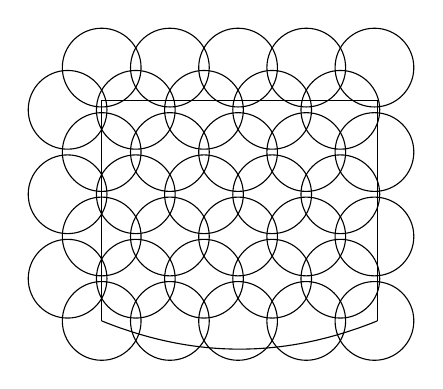
\begin{tikzpicture}[every node/.style={inner sep=0pt},x=1cm,y=1cm]
\begin{scope}[yscale=0.7]
\draw (0,0) to[out=-30,in=-150] (3.5,0);
\draw (3.5,0) to (3.5,4);
\draw (3.5,4) to (0,4);
\draw (0,4) to (0,0);
\foreach \y in {0,...,6}{%
\foreach \x in {0,...,4}{%
\node[circle,draw=black, inner sep=0pt,minimum size=1cm] (b) at ({(\x - Mod(\y,2)/2)*0.866}, \y * 0.766) {};

}
}
\end{scope}
\end{tikzpicture}
\end{document}